\subsection{Short-Time-Fourier-Transformation (STFT)}
\begin{tabular}{ll}
\parbox{5cm}{
    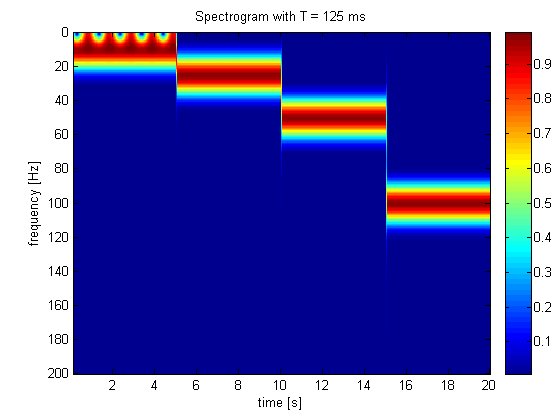
\includegraphics[width=5cm]{Content/STFT/stft.png} \\
    \tiny 4 versch. Cos-Schwingungen nacheinander}
& \parbox{12cm}{
    \begin{liste}
    %\scriptsize 
	 \item STFT unterteilt Signal in Bereiche (Fensterfunktionen) $\Rightarrow$
	 klassische Fourierkoeffizienten
	 \item Weighted Overlap Add (WOLA): Bereiche
     �berlappen sich (Fenster)
     \item Breites Fenster $\Rightarrow$ hohe Frequenzaufl�sung \&
     schlechte Zeitaufl�sung
     \item Schmales Fenster $\Rightarrow$ niedrige Frequenzaufl�sung \&
     hohe Zeitaufl�sung
     \item $X(n, k)$ sind die Signalparameter f�r Fensterposition $n$ \&
     Frequenz $\frac{2\pi k}{N}$
	\end{liste}

    $X(n, k) = \sum\limits^{N-1+n}_{m=n} w(m-n)x(m)e^{-j\Omega_N k(m-n)} = x(n)
    \ast h_w(n,k)$ }
\end{tabular}
%\normalsize

